% Appendices
\appendix
\chapter{System Details}
\section{AR.Drone}
The drone used in this research is the Parrot AR.Drone 2.0 Elite Edition.
It was released by Parrot SA in 2012.
An image is shown in \fref{fig:ardrone}.

\begin{figure}[h]
  \centering
  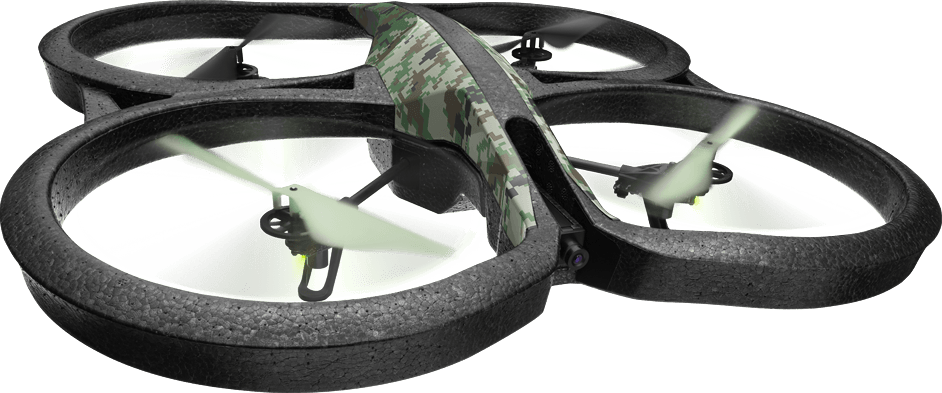
\includegraphics[width=0.5\textwidth]{ardrone}
  \caption[AR.Drone]{AR.Drone 2.0 Elite Edition}
  \label{fig:ardrone}
\end{figure}

Technical specifications are shown in \tref{tab:ardrone_specs}.

\begin{table}[h]
  \centering
  \caption[AR.Drone specifications]{The specifications of the AR.Drone.}
  \begin{tabular}{ll}
    \toprule
    Item & Value \\
    \midrule
    Resolution & 720\,p\\
    Framerate & 30\,fps\\
    Field of view & 92°\\
    Connection & Wi-Fi\\
    Gyroscope  &	3 axles, accuracy of 2,000°/second\\
    Accelerometer  &	3 axles, accuracy of +/- 50\,mg\\
    Magnetometer  &	3 axles, accuracy of 6°\\
    Pressure sensor  & Accuracy of +/- 10\,Pa\\
    Altitude ultrasound sensor  & Measures altitude\\
    Brushless motor power & 14.5\,W\\
    Brushless motor speed & 28,500\,rpm\\
    Weight with indoor frame & 420\,g\\
    \bottomrule
  \end{tabular}
  \label{tab:ardrone_specs}
\end{table}

\section{Motion capture system}
The motion capture system is a set of ten Prime 17W cameras from Optitrack.
One is shown in \fref{fig:mocap_camera}, and technical specifications are in \tref{tab:mocap_specs}.

\begin{figure}[h]
  \centering
  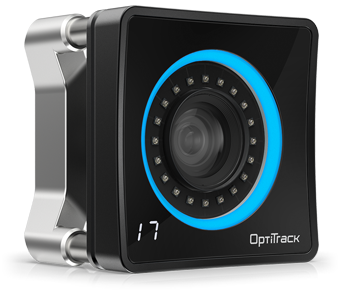
\includegraphics[width=0.5\textwidth]{mocap_camera}
  \caption[Motion capture camera]{The Prime 17W motion capture camera.}
  \label{fig:mocap_camera}
\end{figure}

\begin{table}[h]
  \centering
  \caption[Webcam specifications]{The specifications of the iBuffalo BSW20KM11 webcam.}
  \begin{tabular}{ll}
    \toprule
    Item & Value \\
    \midrule
    Resolution & $1644\times1088$\,pixels\\
    Framerate & 30--360\,fps\\
    Latency & 2.8\,ms\\
    Horizontal field of view & 70°\\
    Vertical field of view & 49°\\
    Filter & 850\,nm band-pass\\
    \bottomrule
  \end{tabular}
  \label{tab:mocap_specs}
\end{table}

\section{Motion capture computer}
The motion capture computer is a Clevo W255HS, running Windows 7 Enterprise.
Its specifications are in \tref{tab:clevo_mocap}.

\begin{table}[h]
  \centering
  \caption[Motion capture computer specifications]{The specifications of the Clevo W255HS computer used to interface with the motion capture system.}
  \begin{tabular}{ll}
    \toprule
    Item & Value \\
    \midrule
    Processor & Intel Core i7-2860QM CPU @ 2.50\,GHz\\
    GPU & nVidia GEFORCE GT 630M, 1\,GB\\
    RAM & 8\,GB\\
    Bits & 64 \\
    \bottomrule
  \end{tabular}
  \label{tab:clevo_mocap}
\end{table}

\section{Operating station}
  The operating station is a Clevo W370ET running Kubuntu 16.10.
  Its specifications are in \tref{tab:clevo_opstn}.

  \begin{table}[h]
    \centering
    \caption[Operating station computer specifications]{The specifications of the Clevo W370ET computer used as the operating station.}
    \begin{tabular}{ll}
      \toprule
      Item & Value \\
      \midrule
      Processor & Intel Core i7-3630QM CPU @ 2.40\,GHz\\
      GPU & nVidia GEFORCE GT 660M, 2\,GB\\
      RAM & 8\,GB\\
      Bits & 64 \\
      \bottomrule
    \end{tabular}
    \label{tab:clevo_opstn}
  \end{table}

\section{Docker environment}
  For the \gls{docker} container that \gls{spirit} runs in, the base is from \texttt{\detokenize{ros:kinetic-robot}}.

  The following ROS packages are installed:

  \begin{itemize}
    \item \textsf{\detokenize{ardrone-autonomy}}
    \item \textsf{\detokenize{image-proc}}
    \item \textsf{\detokenize{mocap_optitrack}}
    \item \textsf{\detokenize{usb_cam}}
  \end{itemize}

  \gls{python} 2.7.13 is installed, with the following dependencies needed for running \gls{spirit}.

  \begin{itemize}
    \item \textsf{\detokenize{catkin_pkg}}
    \item \textsf{\detokenize{defusedxml}}
    \item \textsf{\detokenize{lxml}}
    \item \textsf{\detokenize{numpy}}
    \item \textsf{\detokenize{pygame}}
    \item \textsf{\detokenize{pyyaml}}
    \item \textsf{\detokenize{rospkg}}
    \item \textsf{\detokenize{tqdm}}
  \end{itemize}


\section{External interfaces}
The controller used was an off-the-shelf PlayStation3 controller.

The webcam used to record the experiments was a BSW20KM11 by iBuffalo.
It is shown in \fref{fig:webcam}, and its technical specifications are in \tref{tab:webcam_specs}.

\begin{figure}[h]
  \centering
  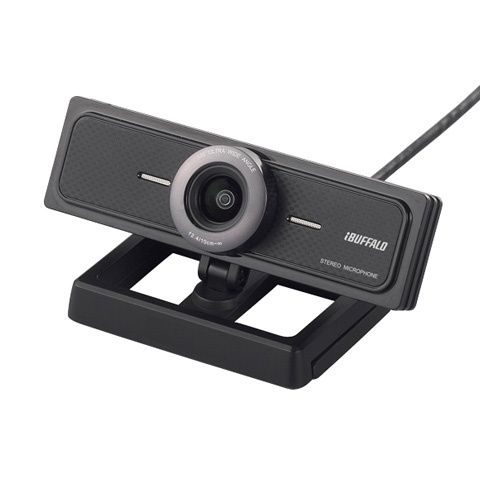
\includegraphics[width=0.5\textwidth]{webcam}
  \caption[Webcam]{The BSW20KM11 webcam.}
  \label{fig:webcam}
\end{figure}

\begin{table}[h]
  \centering
  \caption[Webcam specifications]{The specifications of the iBuffalo BSW20KM11 webcam.}
  \begin{tabular}{ll}
    \toprule
    Item & Value \\
    \midrule
    Resolution & 1080\,p\\
    Framerate & 30\,fps\\
    Field of view & 120°\\
    Microphone & Stereo \\
    \bottomrule
  \end{tabular}
  \label{tab:webcam_specs}
\end{table}
